\documentclass[main.tex]{subfiles}
\begin{document}
\begin{titlingpage}
\begin{center}

~ \\[3cm]

%\includegraphics[width=0.6\textwidth]{figurer/ASE}~\\[1cm]

\textsc{\LARGE Bilag 5}\\[1.5cm]

%\textsc{\Large Sundhedsteknologi}\\
%\textsc{\Large 3. semesterprojekt}\\[0.5cm]

\noindent\makebox[\linewidth]{\rule{\textwidth}{0.4pt}}\\
[0.5cm]{\Huge Arkitektur}
\noindent\makebox[\linewidth]{\rule{\textwidth}{0.4pt}}
\end{center}
\vfill
\begin{center}
{\large 19. december 2017}
\end{center}
\end{titlingpage}

\newpage
\tableofcontents*
\newpage

\chapter{Indledning}



\begin{figure}[H]
\centering
{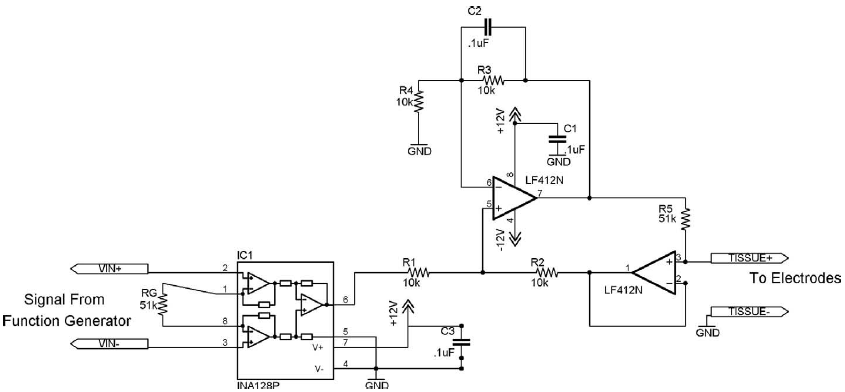
\includegraphics[width=\linewidth]
{Figure/BIdiagram}}
\caption{BI diagram\cite{Aroom2009}}
\label{fig:BIdiagram}
\end{figure}






\chapter{Det oprindelige kredsløb}
\section{Hardware}

\subsection{Strømforsyning}
I artiklen \cite{Aroom2009} blev der brugt en $\pm$12v strømforsyning tilsluttet til netforsyningen. Vi valgte at undgå netforsyningen, ved at sætte otte AA batterier i serie, både for +12v og -12v.


\subsection{Funktionsgenerator}
Analog Discovery blev brugt som funktionsgenerator, da denne er nem og hurtig til at generere signaler. Den ønskede frekvens på 50 kHz blev brugt, da det er en brugt frekvens når der skal måles et synk. Amplituden blev sat til 2v. \cite{Kusuhara2004ImpedanceFunction.}



\subsection{Forstærkning}
Signalet fra Analog Discovery går ind til forstærkeren, hvor der blev brugt en INA128 for at efterligne kredsløbet. Den tilhørende gain modstand på 51kohm blev også brugt, da det giver en fordobling af hvad den tilføres.

\begin{figure}[H]
\centering
{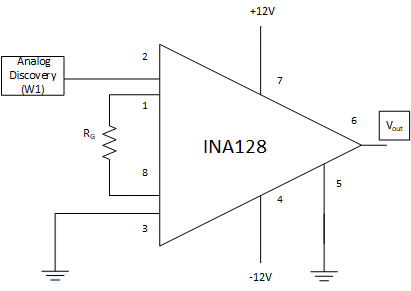
\includegraphics[width=10cm]
{Figure/ina128}}
\caption{Diagram over INA128}
\label{fig:12vbatteri}
\end{figure}







\subsection{Strømgenerator}
\subsection{Elektroder}
\subsection{A/D konverter}
\section{Software}
\subsection{Waveforms}

\section{Testopstillinger}
\section{Konklusion}

\chapter{Det modificeret kredsløb}
\section{Hardware del 1 - Strømgenerator}
\subsection{Strømforsyning}
\subsection{Funktionsgenerator}
\subsection{Forstærkning}
\subsection{Strømgenerator}
\subsection{Elektroder}
\section{Hardware del 2 - Spændingsmåler}
\subsection{Strømforsyning}
\subsection{Elektroder}
\subsection{Forstærkning}
\subsection{Antialiaseringsfilter}
\subsection{A/D konverter}


\section{Software}
\subsection{Matlab}

\section{Testopstillinger}
\section{Konklusion}

\chapter{EMG}


\begin{figure}[H]
\centering
{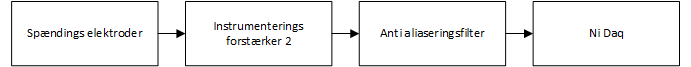
\includegraphics[width=\linewidth]
{Figure/analyse2}}
\caption{Bioimpedans ind}
\label{analyse2}
\end{figure}



\begin{figure}[H]
\centering
{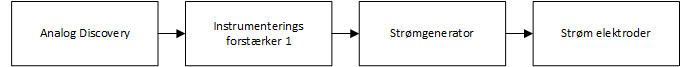
\includegraphics[width=\linewidth]
{Figure/analyse1}}
\caption{Bioimpedans ud}
\label{fig:analyse1}
\end{figure}

Instrumenterings forstærker 1\\
I det oprindelig design af BI konstateret vi at det var lavet lavet til at måle BI'er på skalpen og ikke over svælget. Derfor valgte vi at instrumenterings forstærkeren fik et større signal ind fra Analog Discovery på 2V og 50kHz. I det hele taget undrede vi over artiklens valg af brug af instrumenterings forstærker i starten af kredsløbet, da den ikke er et must for at realisere kredsløbet. Men dens eneste formål var at nedbringe common-mode støj fra funktions generatoren, så vi valgte at beholde denne da vi også vil undgå så meget støj som muligt videre i kredsløbet. Gain var oprindeligt sat til 51 Kohm hvilket giver det dobbelte af hvad instrumenterings forstærkeren tilføre. I diagrammet på figur \ref{BIdiagram} kan det ses at instrumenterings forstærkeren bliver forsynet med +12/-12 V, men der er her valgt at -12 V skal direkte til ground, hvilket har resulteret i at instrumenterings forstærkeren ikke fungerer korrekt, så der er den i stedet forsynet med -12 V og ikke ground.  





Strømgenerator\\
Det forstærket signal som kommer fra udgangen på instrumenterings forstærkeren løber over til strømgeneratoren. Denne strømgenerator er en Howland bridge. Sammensætningen af modstandene er vigtige og deres tolerance skal være lav for at få en korrekt og konstant strøm. For at justerer strømmen kan R5 udskiftes i kredsløbet. For at få en konstant strøm omkring ca. 500 uA, er modstanden ændret fra 51 Kohm til 2 Kohm.  

\textbf{Det oprindelige kredsløb}\\
Først bygges det oprindelige kredsløb som det er opgivet og der bliver foretaget en no load test, for at se om det stemmer overens med figuren fra artiklen.

\begin{figure}[H]
\centering
\begin{minipage}{.5\textwidth}
  \centering
  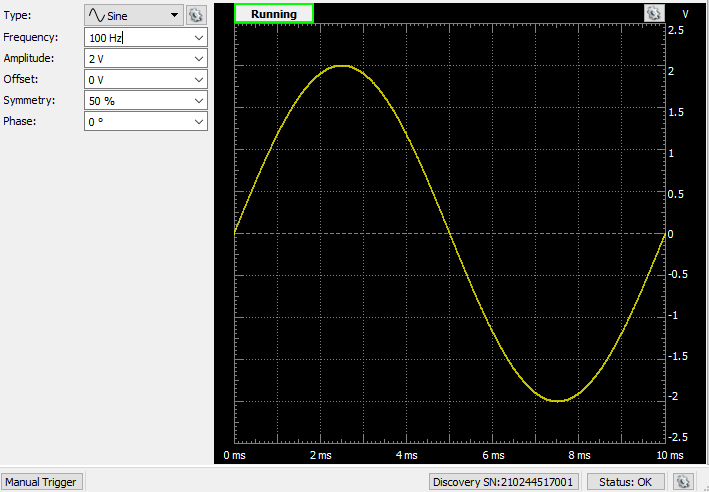
\includegraphics[width=.9\linewidth]{Figure/VCCSwavegen1}
  \captionof{figure}{A figure}
  \label{fig:test1}
\end{minipage}%
\begin{minipage}{.5\textwidth}
  \centering
  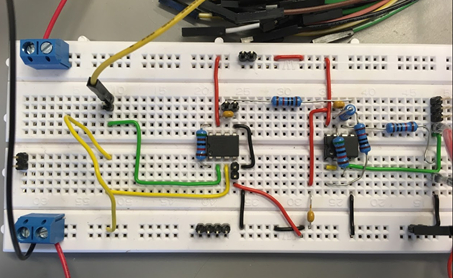
\includegraphics[width=.9\linewidth]{Figure/oprindeligekredslob}
  \captionof{figure}{Another figure}
  \label{fig:test2}
\end{minipage}
\end{figure}



\begin{table}[ht]
\begin{minipage}[b]{0.30\linewidth}
\centering
\begin{tabular}{ r |  r }
    \hline
    Hz & uA \\ \hline
    100 & 49 \\ \hline
    200 & 40 \\ \hline
    300 & 35 \\ \hline
    400 & 32 \\ \hline
    500 & 30 \\ \hline
    600 & 29 \\ \hline
    700 & 28 \\ \hline
    800 & 27 \\ \hline
    900 & 27 \\ \hline
    1000 & 27 \\ \hline
    2000 & 24 \\ \hline
    3000 & 21 \\ \hline
    4000 & 19 \\ \hline
    5000 & 17 \\ \hline
    6000 & 14 \\ \hline
    7000 & 12 \\ \hline
    8000 & 10 \\ \hline
    9000 & 7 \\ \hline
    10000 & 5 \\ \hline
    20000 & 0 \\ \hline
\end{tabular}
    \caption{Student Database}
    \label{table:student}
\end{minipage}\hfill
\begin{minipage}[b]{0.7\linewidth}
\centering
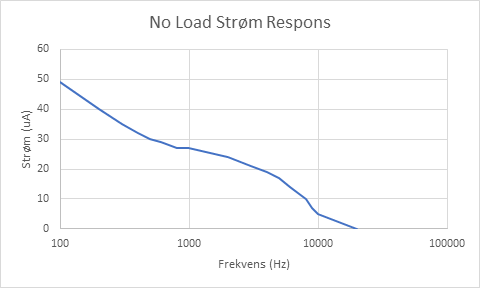
\includegraphics[width=10cm]{Figure/stromfrekvensoprindelig}
\captionof{figure}{2-D scatterplot of the Student Database}
\label{fig:image}
\end{minipage}
\end{table}


\textbf{Det modificeret kredsløb}\\

\begin{table}[H]
\begin{minipage}[b]{0.30\linewidth}
\centering
\begin{tabular}{ r |  r }
    \hline
    Hz & uA \\ \hline
    100 & 1268 \\ \hline
    200 & 1051 \\ \hline
    300 & 920 \\ \hline
    400 & 845 \\ \hline
    500 & 802 \\ \hline
    600 & 775 \\ \hline
    700 & 756 \\ \hline
    800 & 744 \\ \hline
    900 & 735 \\ \hline
    1000 & 728 \\ \hline
    2000 & 703 \\ \hline
    3000 & 696 \\ \hline
    4000 & 692 \\ \hline
    5000 & 688 \\ \hline
    6000 & 685 \\ \hline
    7000 & 683 \\ \hline
    8000 & 680 \\ \hline
    9000 & 678 \\ \hline
    10000 & 676 \\ \hline
    20000 & 675 \\ \hline
    30000 & 634 \\ \hline
    40000 & 596 \\ \hline
    50000 & 542 \\ \hline
    60000 & 475 \\ \hline
    70000 & 405 \\ \hline
    80000 & 332 \\ \hline
    90000 & 268 \\ \hline
    100000 & 210 \\ \hline
    110000 & 161 \\ \hline
    120000 & 120 \\ \hline
    130000 & 87 \\ \hline
    140000 & 60 \\ \hline
    150000 & 40 \\ \hline
    160000 & 25 \\ \hline
    170000 & 16 \\ \hline
    180000 & 10 \\ \hline
    190000 & 6 \\ \hline
    200000 & 4 \\ \hline
    210000 & 2 \\ \hline
    220000 & 1 \\ \hline
    230000 & 1 \\ \hline
    240000 & 0 \\ \hline
        
\end{tabular}
    \caption{Student Database}
    \label{table:student}
\end{minipage}\hfill
\begin{minipage}[b]{0.7\linewidth}
\centering
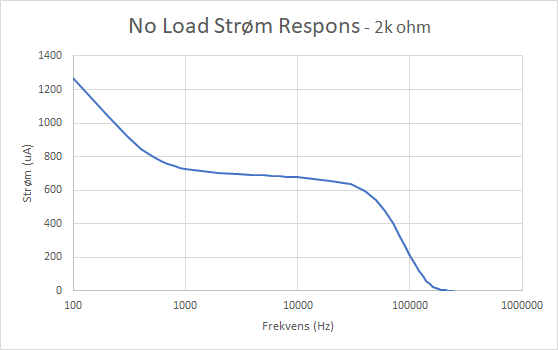
\includegraphics[width=10cm]{Figure/stromfrekvensoprindelig2k}
\captionof{figure}{2-D scatterplot of the Student Database}
\label{fig:image}
\end{minipage}
\end{table}














Overvejelser om mulige løsninger
løsninger I har valgt, begrundelsen herfor
grundlæggende valg af hardware- og softwaremæssige komponenter, som er kritiske for realisering af systemet

For at træffe et valg kan der analyseres og diskuteres forskellige løsninger mht. til ydeev-ne, pris, leveringstid og forhåndskendskab. Disse kan med fordel opstilles i tabelform.

Anti-alisering
Elektroder
Konstant strøm
Lavpas filtering
Ensretter
Sampling af signal






\chapter{Konklusion}

\bibliography{Mendeley.bib}
\end{document}


